%%
%% Automatically generated file from DocOnce source
%% (https://github.com/hplgit/doconce/)
%%
%%
% #ifdef PTEX2TEX_EXPLANATION
%%
%% The file follows the ptex2tex extended LaTeX format, see
%% ptex2tex: http://code.google.com/p/ptex2tex/
%%
%% Run
%%      ptex2tex myfile
%% or
%%      doconce ptex2tex myfile
%%
%% to turn myfile.p.tex into an ordinary LaTeX file myfile.tex.
%% (The ptex2tex program: http://code.google.com/p/ptex2tex)
%% Many preprocess options can be added to ptex2tex or doconce ptex2tex
%%
%%      ptex2tex -DMINTED myfile
%%      doconce ptex2tex myfile envir=minted
%%
%% ptex2tex will typeset code environments according to a global or local
%% .ptex2tex.cfg configure file. doconce ptex2tex will typeset code
%% according to options on the command line (just type doconce ptex2tex to
%% see examples). If doconce ptex2tex has envir=minted, it enables the
%% minted style without needing -DMINTED.
% #endif

% #define PREAMBLE

% #ifdef PREAMBLE
%-------------------- begin preamble ----------------------

\documentclass[%
twoside,                 % oneside: electronic viewing, twoside: printing
final,                   % or draft (marks overfull hboxes, figures with paths)
10pt]{article}

\listfiles               % print all files needed to compile this document

\usepackage{relsize,makeidx,color,setspace,amsmath,amsfonts}
\usepackage[table]{xcolor}
\usepackage{bm,microtype}

\usepackage{graphicx}

\usepackage{ptex2tex}
% #ifdef MINTED
\usepackage{minted}
\usemintedstyle{default}
% #endif

\usepackage[T1]{fontenc}
%\usepackage[latin1]{inputenc}
\usepackage{ucs}
\usepackage[utf8x]{inputenc}

\usepackage{lmodern}         % Latin Modern fonts derived from Computer Modern

% Hyperlinks in PDF:
\definecolor{linkcolor}{rgb}{0,0,0.4}
\usepackage{hyperref}
\hypersetup{
    breaklinks=true,
    colorlinks=true,
    linkcolor=linkcolor,
    urlcolor=linkcolor,
    citecolor=black,
    filecolor=black,
    %filecolor=blue,
    pdfmenubar=true,
    pdftoolbar=true,
    bookmarksdepth=3   % Uncomment (and tweak) for PDF bookmarks with more levels than the TOC
    }
%\hyperbaseurl{}   % hyperlinks are relative to this root

\setcounter{tocdepth}{2}  % number chapter, section, subsection

% Tricks for having figures close to where they are defined:
% 1. define less restrictive rules for where to put figures
\setcounter{topnumber}{2}
\setcounter{bottomnumber}{2}
\setcounter{totalnumber}{4}
\renewcommand{\topfraction}{0.85}
\renewcommand{\bottomfraction}{0.85}
\renewcommand{\textfraction}{0.15}
\renewcommand{\floatpagefraction}{0.7}
% 2. ensure all figures are flushed before next section
\usepackage[section]{placeins}
% 3. enable begin{figure}[H] (often leads to ugly pagebreaks)
%\usepackage{float}\restylefloat{figure}

% prevent orhpans and widows
\clubpenalty = 10000
\widowpenalty = 10000

\newenvironment{doconceexercise}{}{}
\newcounter{doconceexercisecounter}
% --- begin definition of \listofexercises command ---
\makeatletter
\newcommand\listofexercises{\section*{List of Exercises and Projects}
\@starttoc{loe}
}
\newcommand*{\l@doconceexercise}{\@dottedtocline{0}{0pt}{6.5em}}
\makeatother
% --- end definition of \listofexercises command ---



% ------ header in subexercises ------
%\newcommand{\subex}[1]{\paragraph{#1}}
%\newcommand{\subex}[1]{\par\vspace{1.7mm}\noindent{\bf #1}\ \ }
\makeatletter
% 1.5ex is the spacing above the header, 0.5em the spacing after subex title
\newcommand\subex{\@startsection{paragraph}{4}{\z@}%
                  {1.5ex\@plus1ex \@minus.2ex}%
                  {-0.5em}%
                  {\normalfont\normalsize\bfseries}}
\makeatother


% --- end of standard preamble for documents ---


% insert custom LaTeX commands...

\raggedbottom
\makeindex

%-------------------- end preamble ----------------------

\begin{document}

% endif for #ifdef PREAMBLE
% #endif


% ------------------- main content ----------------------

% Slides for many-body text


% ----------------- title -------------------------

\thispagestyle{empty}

\begin{center}
{\LARGE\bf
\begin{spacing}{1.25}
Projects and how do develop a numerical project
\end{spacing}
}
\end{center}

% ----------------- author(s) -------------------------

\begin{center}
{\bf Carlo Barbieri, Wim Dickhoff, Gaute Hagen, Morten Hjorth-Jensen, and Artur Polls${}^{}$} \\ [0mm]
\end{center}

    \begin{center}
% List of all institutions:
\end{center}
    
% ----------------- end author(s) -------------------------

\begin{center} % date
July 6-24, Ganil, Caen, France
\end{center}

\vspace{1cm}


\tableofcontents


\vspace{1cm} % after toc




\subsection{Plan for the Talent course}
An essential element of the Talent courses is to develop a large project(s) which allows you to study and understand
teoretical concepts in nuclear physics.  
These concepts will in turn allow you to interpret results from experiments and understand the pertinent physics in terms of the underlying forces and laws of motion.

Together with the regular lectures in the morning, the hope is that
during these three weeks you will be able to write and run a program
which implements at least one of the methods discussed during the
lectures.  The lectures will also cover additional material which aims
at giving you a broader view on what can be achieved with the methods
to be discussed. Combined with the 'hands-on' afternoon sessions, the
hope is that the lectures and the computational projects will together
allow you to achieve these goals. For those of you who would like to
get credits to be transferred to your home university, the project(s)
can be extended upon allowing you to include further elements to the
many-body methods. The load of the final project is estimated to be 
80 hours. In total, attendence at the course and doing
the final project amounts to seven ECTS. There is no credit transfer
for Northern-American students.

\subsection{Outline of the project(s)}

What is outlined here are several paths that will allow you to develop
a program which can be used to study nuclear systems. In particular,
we will focus on two widely used many-body methods, coupled cluster
theory with its various approximations and Green's function theory.

Before we begin, we would however like to present a warm-up problem which 
contains
many of the basic elements of the many-body methods exposed in this course. Furthermore, the simple pairing 
model described below, provides us with  benchmark results to which we can compare 
the different many-body methods. The basic elements of the model (single-particle basis and Hamiltonian)
can easily be (if structured properly in your program) extended to studies of more realistic systems, either 
finite systems like nuclei or infinite nuclear matter. 

The first part of the project is a traditional paper and pencil part, where the aim is to 
apply second quantization in order to set up the Hamiltonian matrix to be diagonalized.
We will study this model the first two afternoons of the school. 

At most, with four particles in four doubly degenerate single particle states and no broken pairs,
you will have a $6 \times 6$ Hamiltonian matrix to diagonalize. Below, you will find a simple python program
which performs the diagonalization and plots the eigenvalues. Parts of this warm-up exercise are solved below. 
These aspects will be discussed partly during the lectures but also during some of the afternoon sessions.
Practical guidelines for code writing will also be discussed.


This exercise will allow us to start writing our first skeleton for a coupled cluster theory program at the so-called doubles level of truncation. It will also, for those of you who will prefer  to study Green's functions, serve as a 
starting point for developing the skeleton of a program for this method. The aim is to finish this part of the program during the first week.

With a program which then benchmarks the simple pairing model, we will turn our attention to more realistic systems.
Here we propose the following  paths that can be studied with either coupled cluster theory or Green's function theory. Many of the technicalities will be discussed at the lectures and the afternoon sessions during the last two weeks.

\begin{enumerate}
\item Studies of nuclear matter with a cartesian basis using coupled cluster theory at the level of doubles excitations
\begin{itemize}

  \item During the three weeks of the course we will mainly focus on two-particle and two-hole excitations 

  \item Focusing only on two-particle correlations in a finite cartesian basis, these can be compared with Brueckner-Hartree-Fock calculations in the infinite limit. The latter should represent numerically exactly two-particle correlations to infinite order. A simple model for the nuclear force will be used.

  \item For the final project the code can be extended to include particle-hole correlations as well

\end{itemize}

\noindent
\item Studies of finite nuclei using coupled cluster theory at the level of doubles excitations only
\begin{itemize}

  \item Here we will provide Hartree-Fock based single-particle states and two-body interactions in an uncoupled scheme.

  \item The system to be studied is that of neutrons in harmonic oscillator traps. 

  \item For the final project, one can include singles excitations as well.

\end{itemize}

\noindent
\item The two above paths can be performed using Green's function as well.
\begin{itemize}

  \item Studies of infinite nuclear matter including two-particle and two-hole correlations using a cartesian basis.

  \item Comparison of two-particle correlations from Brueckner-Hartree-Fock calculations in the infinite limit

\end{itemize}

\noindent
\item Studies of finite nuclei with the Green's function method
\begin{itemize}

  \item Again we will provide Hartree-Fock based single-particle states and two-body interactions in an uncoupled scheme.

  \item The system to be studied is that of neutrons in harmonic oscillator traps. 

  \item For the final project, one can include self-consistently calculated single-particle energies as well.
\end{itemize}

\noindent
\end{enumerate}

\noindent
When working on the projects, we recommend strongly that you form teams of two-three participants. Every team
\textbf{must} have a \emph{github account} where we can monitor your progress and give you appropriate feedback.

If you have not used version control before now, it is time to do so. 
Proper version control is central to a good ethical scientific conduct. 
We do require that you use some kind of version control software when working on the projects. We recommend strongly \href{{https://github.com/}}{github}. 

Furthermore, before coming to the course, we recommend that you refresh your knowledge on second quantization.
If your background in second quantization is rudimentary and mentioning of Wick's leave you gazing at the stars,
we recommend that you study the material at the course web site on \href{{http://nucleartalent.github.io/Course2ManyBodyMethods/doc/pub/secondquant/html/secondquant-bs.html}}{second quantization}. Try in particular to do some of the exercises.

We will also require that you come with your own laptop and have installed either a
\begin{itemize}
\item Fortran compiler or a 

\item c++ compiler
\end{itemize}

\noindent
You can use Python as programming language as well, but normally the efficiency of Python for the problems addressed in this course is lower than for codes written in Fortran or c++. We recommend however that use Python as a scripting language for running codes and making plots, as well as using the ipython notebooks provided by us.  

\subsection{Some basic ingredients for a successful numerical project}

In when building up a numerical project there are several elements you should think of
\begin{enumerate}
  \item How to structure a code in terms of functions

  \item How to make a module

  \item How to read input data flexibly from the command line

  \item How to create graphical/web user interfaces

  \item How to write unit tests (test functions or doctests)

  \item How to refactor code in terms of classes (instead of functions only), in our case you think of a system and a solver class

  \item How to conduct and automate large-scale numerical experiments

  \item How to write scientific reports in various formats ({\LaTeX}, HTML)
\end{enumerate}

\noindent
The conventions and techniques outlined here will save you a lot of time when you incrementally extend software over time from simpler to more complicated problems. In particular, you will benefit from many good habits:
\begin{enumerate}
\item New code is added in a modular fashion to a library (modules)

\item Programs are run through convenient user interfaces

\item It takes one quick command to let all your code undergo heavy testing 

\item Tedious manual work with running programs is automated,

\item Your scientific investigations are reproducible, scientific reports with top quality typesetting are produced both for paper and electronic devices.
\end{enumerate}

\noindent
\subsection{The pairing model as warm-up problem}

We present a simplified Hamiltonian consisting of an unperturbed
Hamiltonian and a so-called pairing interaction term. It is a model
which to a large extent mimicks some central features of atomic
nuclei, certain atoms and systems which exhibit superfluiditity or
superconductivity.  To study this system, we will use a mix of
many-body perturbation theory (MBPT), Hartree-Fock (HF) theory and full
configuration interaction (FCI) theory. The latter will also provide us with
the exact answer.  When setting up the Hamiltonian matrix you will
need to solve an eigenvalue problem.

We define first the Hamiltonian, with a definition of the model space
and the single-particle basis. Thereafter, we present the various
exercises.


The Hamiltonian acting in the complete Hilbert space (usually infinite
dimensional) consists of an unperturbed one-body part, $\hat{H}_0$,
and a perturbation $\hat{V}$.

We limit ourselves to at most two-body interactions, our Hamiltonian
is then represented by the following operators
\[
\hat{H} = \sum_{\alpha\beta}\langle \alpha |h_0|\beta\rangle
a_{\alpha}^{\dagger}a_{\beta}
+\frac{1}{4}\sum_{\alpha\beta\gamma\delta}\langle \alpha\beta|
V|\gamma\delta\rangle
a_{\alpha}^{\dagger}a_{\beta}^{\dagger}a_{\delta}a_{\gamma},
\]
where $a_{\alpha}^{\dagger}$ and $a_{\alpha}$ etc.~are standard
fermion creation and annihilation operators, respectively, and
$\alpha\beta\gamma\delta$ represent all possible single-particle
quantum numbers.  The full single-particle space is defined by the
completeness relation 
\[
\hat{{\bf 1}} = \sum_{\alpha=1}^{\infty}|\alpha \rangle \langle \alpha|.
\]
In our calculations
we will let the single-particle states $|\alpha\rangle$ be
eigenfunctions of the one-particle operator $\hat{h}_0$. Note that the two-body part of the Hamiltonian 
contains anti-symmetrized matrix elements.


The above Hamiltonian acts in turn on various many-body Slater
determinants constructed from the single-basis defined by the one-body
operator $\hat{h}_0$.  As an example, the two-particle model space
$\mathcal{P}$ is defined by an operator
\[
\hat{P} = \sum_{\alpha\beta =1}^{m}|\alpha\beta \rangle \langle
\alpha\beta|,
\]
where we assume that $m=\dim(\mathcal{P})$ and the full space is
defined by
\[
\hat{P}+\hat{Q}=\hat{{\bf 1}},
\]
with the projection operator
\[
\hat{Q} = \sum_{\alpha\beta =m+1}^{\infty}|\alpha\beta \rangle \langle
\alpha\beta|,
\]
being the complement of $\hat{P}$.


Our specific model consists of $N$ doubly-degenerate and equally
spaced single-particle levels labelled by $p=1,2,\dots$ and spin
$\sigma=\pm 1$.  These states are schematically portrayed in
Fig.~ref{fig:schematic}.  The first two single-particle levels define
a possible model space, indicated by the label $\mathcal{P}$.  The
remaining states span the excluded space $\mathcal{Q}$.

We write the Hamiltonian as
\[ \hat{H} = \hat{H}_0 + \hat{V} , \]
where
\[
\hat{H}_0=\xi\sum_{p\sigma}(p-1)a_{p\sigma}^{\dagger}a_{p\sigma}
\]
and
\[
\hat{V}=-\frac{1}{2}g\sum_{pq}a^{\dagger}_{p+}
a^{\dagger}_{p-}a_{q-}a_{q+}.
\]
Here, $H_0$ is the unperturbed Hamiltonian with a spacing between
successive single-particle states given by $\xi$, which we will set to
a constant value $\xi=1$ without loss of generality. The two-body
operator $\hat{V}$ has one term only. It represents the pairing
contribution and carries a constant strength $g$.

The indices
$\sigma=\pm$ represent the two possible spin values. The interaction
can only couple pairs and excites therefore only two particles at the
time, as indicated by the rightmost four-particle state in
Fig.~ref{fig:schematic}. There one of the pairs is excited to the
state with $p=9$ and the other to the state $p=7$. The two middle
possibilities are not possible with the present model.  We label
single-particle states within the model space as hole-states. The
single-particle states outside the model space are then particle
states. 

In our model we have kept both the interaction strength and the
single-particle level as constants.  In a realistic system like an
atom or the atomic nucleus this is not the case.


\begin{figure}[t]
  \centerline{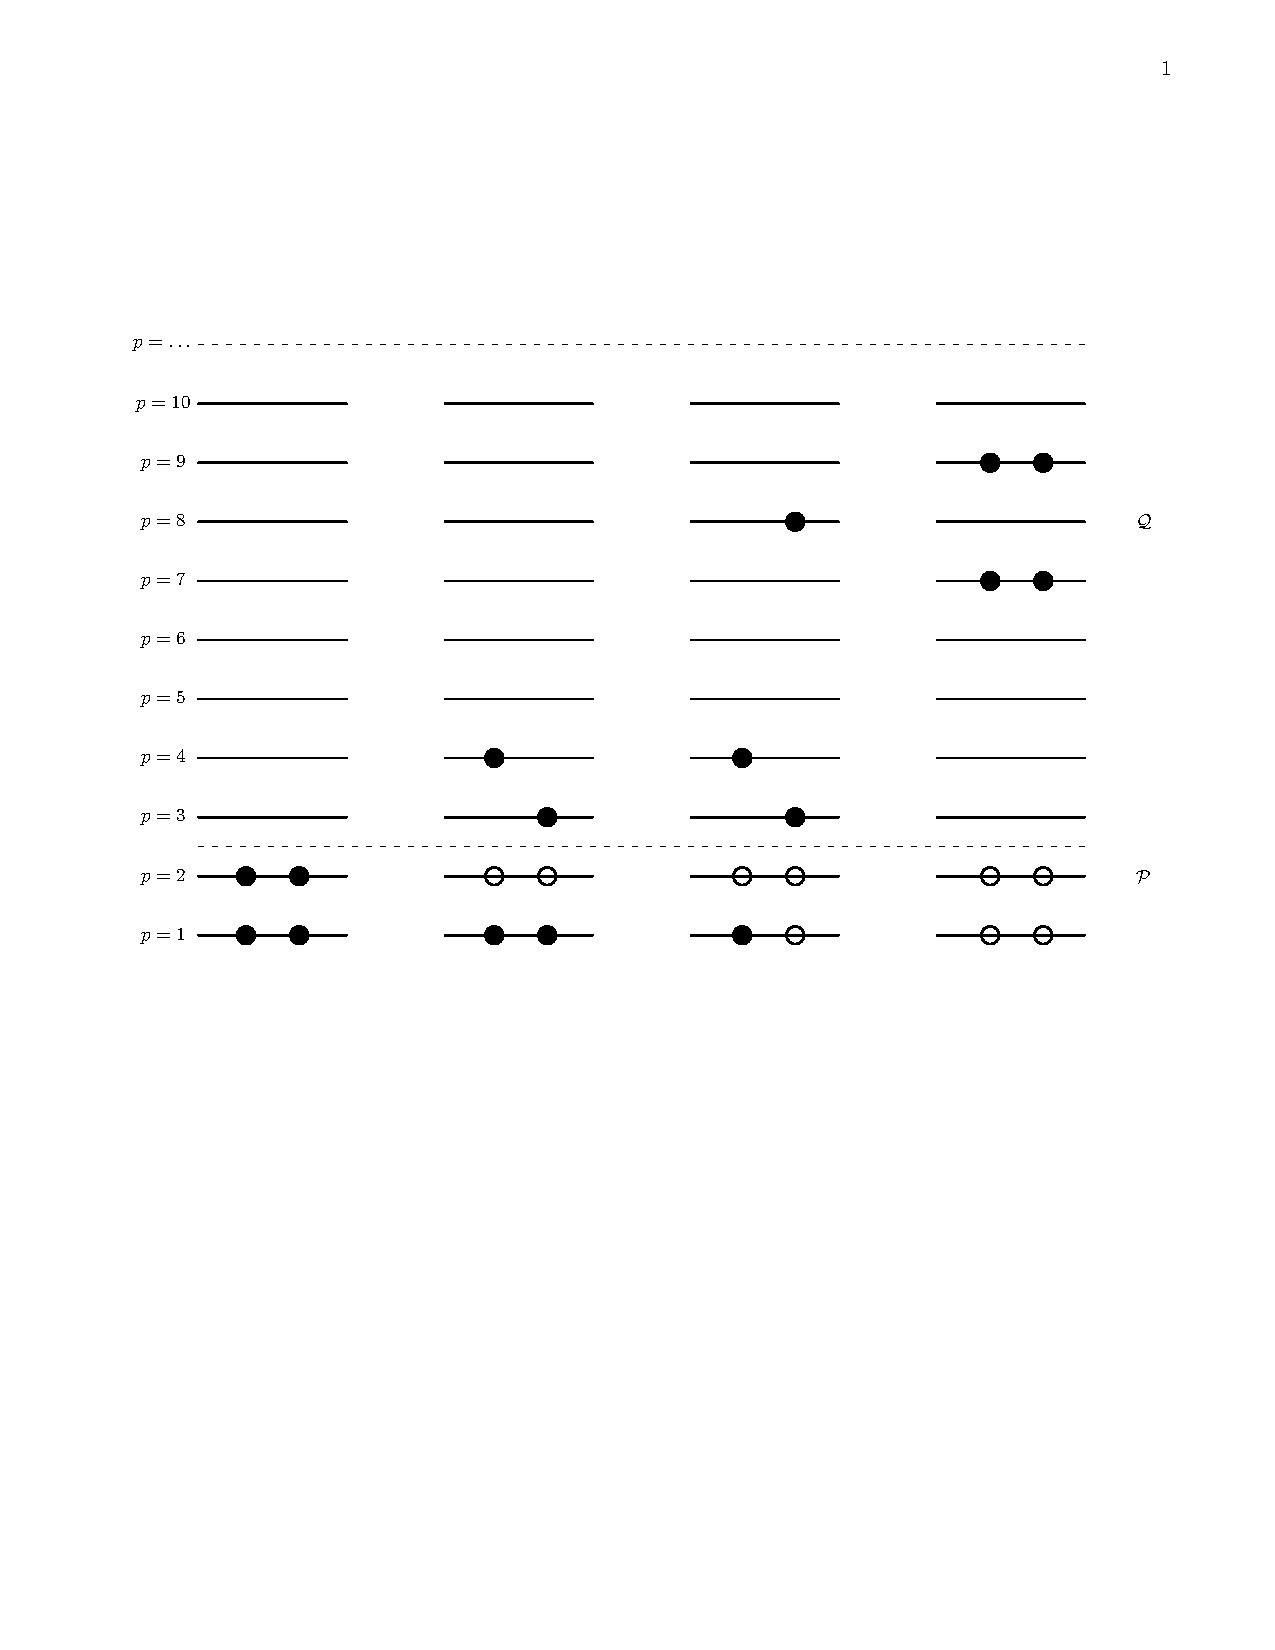
\includegraphics[width=0.7\linewidth]{fig-proj/simplemodel.pdf}}
  \caption{
  Schematic plot of the possible single-particle levels with double degeneracy.  The filled circles indicate occupied particle  states while the empty circles represent vacant particle(hole)  states.  The spacing between each level $p$ is constant in this picture.  The first two single-particle levels define our possible  model space, indicated by the label $\mathcal{P}$.  The remaining  states span the excluded space $\mathcal{Q}$.  The first state to  the left represents a possible ground state representation for a  four-fermion system. In the second state to the left, one pair is   broken. This possibility is however not included in our  interaction. \label{fig:schematic}
  }
\end{figure}
%\clearpage % flush figures fig:schematic




% --- begin exercise ---
\begin{doconceexercise}
\refstepcounter{doconceexercisecounter}

\subsection*{Exercise \thedoconceexercisecounter: Pairing Hamiltonian}



\subex{a)}
Show that the unperturbed Hamiltonian $\hat{H}_0$ and $\hat{V}$
  commute with both the spin projection $\hat{S}_z$ and the total spin
  $\hat{S}^2$, given by
\[
  \hat{S}_z := \frac{1}{2}\sum_{p\sigma} \sigma
  a^\dag_{p\sigma}a_{p\sigma}
\]
and
\[
  \hat{S}^2 := \hat{S}_z^2 + \frac{1}{2}(\hat{S}_+\hat{S}_- +
  \hat{S}_-\hat{S}_+),
\]
where
\[
  \hat{S}_\pm := \sum_{p} a^\dag_{p\pm} a_{p\mp}.
\]
This is an important feature of our system that allows us to
block-diagonalize the full Hamiltonian. We will focus on total spin
$S=0$.  In this case, it is convenient to define the so-called pair
creation and pair annihilation operators
\[
\hat{P}^{+}_p = a^\dag_{p+}a^\dag_{p-},
\]
and
\[
\hat{P}^{-}_p = a_{p-}a_{p+},
\] 
respectively.

Show that you can rewrite the Hamiltonian (with $\xi=1$) as
\[
\hat{H}=\sum_{p\sigma}(p-1)a_{p\sigma}^{\dagger}a_{p\sigma}
-\frac{1}{2}g\sum_{pq}\hat{P}^{+}_p\hat{P}^{-}_q.
\]
Show also that Hamiltonian commutes with the product of the pair
creation and annihilation operators.  This model corresponds to a
system with no broken pairs. This means that the Hamiltonian can only
link two-particle states in so-called spin-reversed states.


\subex{b)}
Construct thereafter the Hamiltonian matrix for a system with no
  broken pairs and total spin $S=0$ for the case of the four lowest
  single-particle levels indicated in the
  Fig.~ref{fig:schematic}. Our system consists of four particles
  only.  Our single-particle space consists of only the four lowest
  levels $p=1,2,3,4$.  You need to set up all possible Slater
  determinants.  Find all eigenvalues by diagonalizing the Hamiltonian
  matrix.  Vary your results for values of $g\in [-1,1]$.  We refer to
  this as the exact calculation. Comment the behavior of the ground
  state as function of $g$.


% --- begin solution of exercise ---
\paragraph{Solution.}
When calculating the matrix elements, we see that we can either have no non-coincidences, two non-coincidences or four non-coincidences. Another way to state this is to say that there can a mismatch of zero, one or two pairs. 

The following python program diagonalizes the above Hamiltonian matrix for a given span of interaction strength values.
\bpypro
from numpy import *
from sympy import *
from matplotlib.pyplot import *


g_array = linspace(-1, 1, 1001)
e1_array = []
e2_array = []

for g in g_array:
	H1 = matrix([[2-g , -g/2.,  -g/2., -g/2., -g/2.,     0], 
		        [-g/2.,   4-g,  -g/2., -g/2.,    0., -g/2.],
		        [-g/2., -g/2.,    6-g,     0, -g/2., -g/2.],
				[-g/2., -g/2.,      0,   6-g, -g/2., -g/2.],
				[-g/2.,     0,  -g/2., -g/2.,   8-g, -g/2.],
				[0    , -g/2.,  -g/2., -g/2., -g/2.,  10-g]]) 

	H2 = matrix([[2-g , -g/2.,  -g/2., -g/2., -g/2.], 
		        [-g/2.,   4-g,  -g/2., -g/2.,    0.],
		        [-g/2., -g/2.,    6-g,     0, -g/2.],
				[-g/2., -g/2.,      0,   6-g, -g/2.],
				[-g/2.,     0,  -g/2., -g/2.,   8-g]]) 

		

	u1, v1 = linalg.eig(H1)
	u2, v2 = linalg.eig(H2)

	if g == 1./2:
		print argmin(u1)

		for i in range(5):
			print " %.3f " % v2[i,0],



	e1_array.append(min(u1))
	e2_array.append(min(u2))


plot(g_array, e1_array, linewidth=2.0)
#plot(g_array, e2_array, linewidth=2.0)
plot(g_array, (2-g_array), linewidth=2.0)
grid()
xlabel(r"Strength of interaction, $g$", fontsize=16)
ylabel(r'Ground state energy', fontsize=16)
#axis([-1,1,-0.4,0.05])
legend(['FCI -- Exact', 'Reference energy'])
savefig("pairing.pdf")
show()
\epypro

% --- end solution of exercise ---

\subex{c)}
Instead of setting up all possible Slater determinants, construct only
an approximation to the ground state (where we assume that the four
particles are in the two lowest single-particle orbits only) which
includes at most two-particle-two-hole excitations. Diagonalize this
matrix and compare with the exact calculation and comment your
results. Can you set up which diagrams this approximation corresponds
to?


\subex{d)}
We switch now to approximative methods, in our case Hartree-Fock
  theory and many-body perturbation theory. Hereafter we will define
  our model space to consist of the single-particle levels $p=1,2$.
  The remaining levels $p=3,4$ define our excluded space.  This means
  that our ground state Slater determinant consists of four particles
  which can be placed in the doubly degenerate orbits $p=1$ and $p=2$.
  Our first step is to perform a Hartree-Fock calculation with the
  pairing Hamiltonian.  Write first the normal-ordered Hamiltonian
  with respect to the above reference state given by four spin $1/2$
  fermions in the single-particle levels $p=1,2$. Define what is meant
  by a canonical Hartree-Fock case, a non-canonical case and a general
  case.  For all three cases, write down the normal-ordered
  Hamiltonian and draw the diagrammatic form of the Hamiltonian for all three cases.



\subex{e)}
We will now set up the Hartree-Fock equations by varying the
coefficients of the single-particle functions. The single-particle
basis functions are defined as
\[
\psi_p = \sum_{\lambda} C_{p\lambda}\psi_{\lambda}.
\]
where in our case $p=1,2,3,4$ and $\lambda=1,2,3,4$, that is the first
four lowest single-particle orbits of Fig.~ref{fig:schematic}.  Set
up the Hartree-Fock equations for this system by varying the
coefficients $C_{p\lambda}$ and solve them for values of $g\in
[-1,1]$.  Comment your results and compare with the exact
solution. Discuss also which diagrams in Fig.~ref{fig:diagrams} that
can be affected by a Hartree-Fock basis. Compute the total binding
energy using a Hartree-Fock basis and comment your results.



\subex{f)}
We will now study the system using non-degenerate
Rayleigh-Schroedinger perturbation theory to third order in the
interaction.  If we exclude the first order contribution, all possible
diagrams (so-called anti-symmetric Goldstone diagrams) are
shown in Fig.~ref{fig:diagrams}.


\begin{figure}[t]
  \centerline{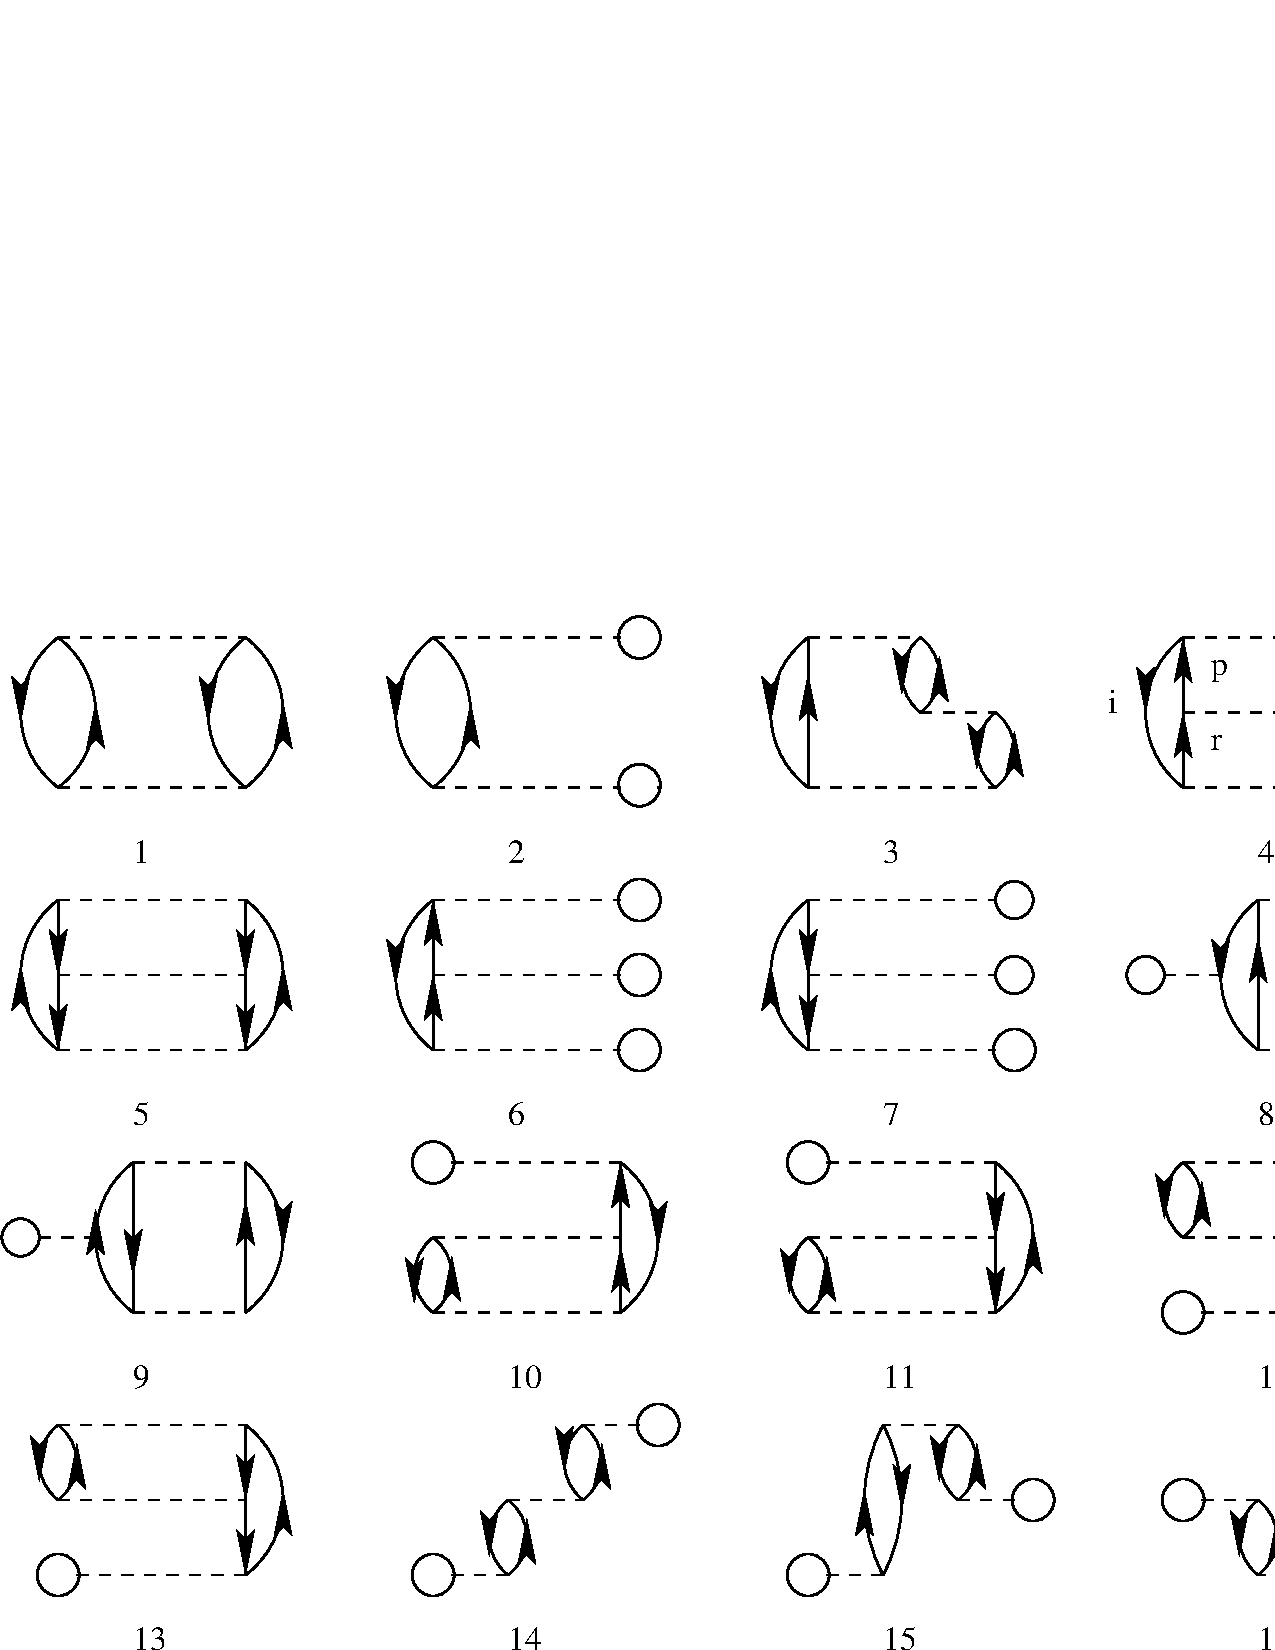
\includegraphics[width=1.0\linewidth]{fig-proj/diagrams.pdf}}
  \caption{
  Diagrams to third order in the interaction, including also non-canonical Hartree-Fock diagrams. The first order term is excluded. All interaction vertices represent anti-symmetrized matrix elements. \label{fig:diagrams}}
  }
\end{figure}
%\clearpage % flush figures fig:diagrams


Based on the form of the interaction, which diagrams contribute to the
binding energy of the ground state?  Write down the expressions for
the diagrams that contribute and find the contribution to the ground
state energy as function $g\in [-1,1]$. Comment your results.  Compare
these results with those you obtained from the exact diagonalization with and without the $4p-4h$ state.
Discuss your results for a canonical Hartree-Fock basis and a non-canonical Hartree-Fock basis.

\subex{g)}
Diagram 1 in Fig.~ref{fig:diagrams} represents a second-order contribution to the energy and a so-called $2p-2h$ contribution to the intermediate states. Write down the expression for the wave operator in this case and compare the possible contributions with the configuration interaction calculations without the $4p-4h$ Slater determinant. Comment your results for 
various values of $g\in [-1,1]$.

\subex{h)}
We limit now the discussion to the canonical Hartree-Fock case only. To fourth order in perturbation theory we can produce diagrams with $1p-1h$ intermediate excitations as shown in Fig.~ref{fig:fourthorder1p1h}, $2p-2h$ excitations, see Fig.~ref{fig:fourthorder2p2h}, $3p-3h$ excitations as shown in Fig.~ref{fig:fourthorder3p3h} and finally so-called diagrams with intermediate four-particle-four-hole excitations, see Fig.~ref{fig:fourthorder4p4h}. 


\begin{figure}[t]
  \centerline{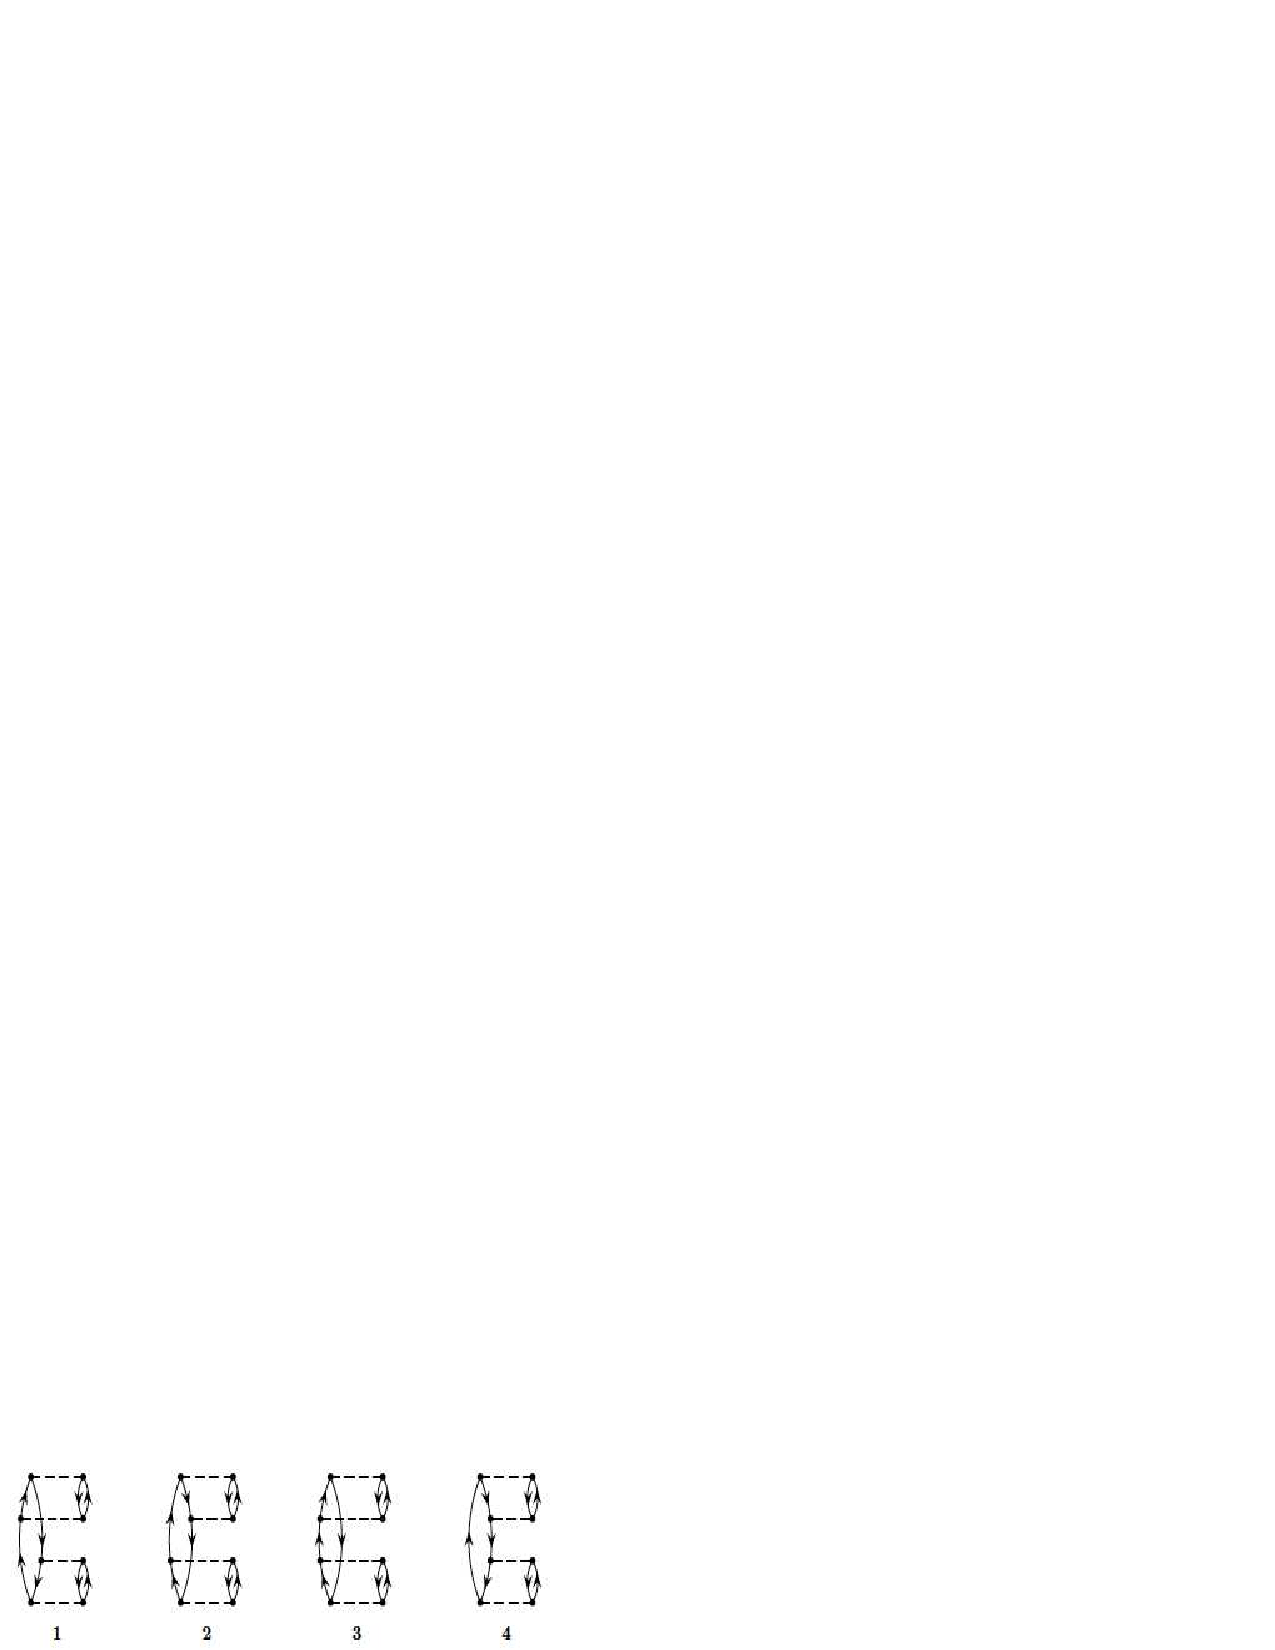
\includegraphics[width=0.6\linewidth]{fig-proj/1p1h.pdf}}
  \caption{
  One-particle-one-hole excitations to fourth order. \label{fig:fourthorder1p1h}
  }
\end{figure}
%\clearpage % flush figures fig:fourthorder1p1h



\begin{figure}[t]
  \centerline{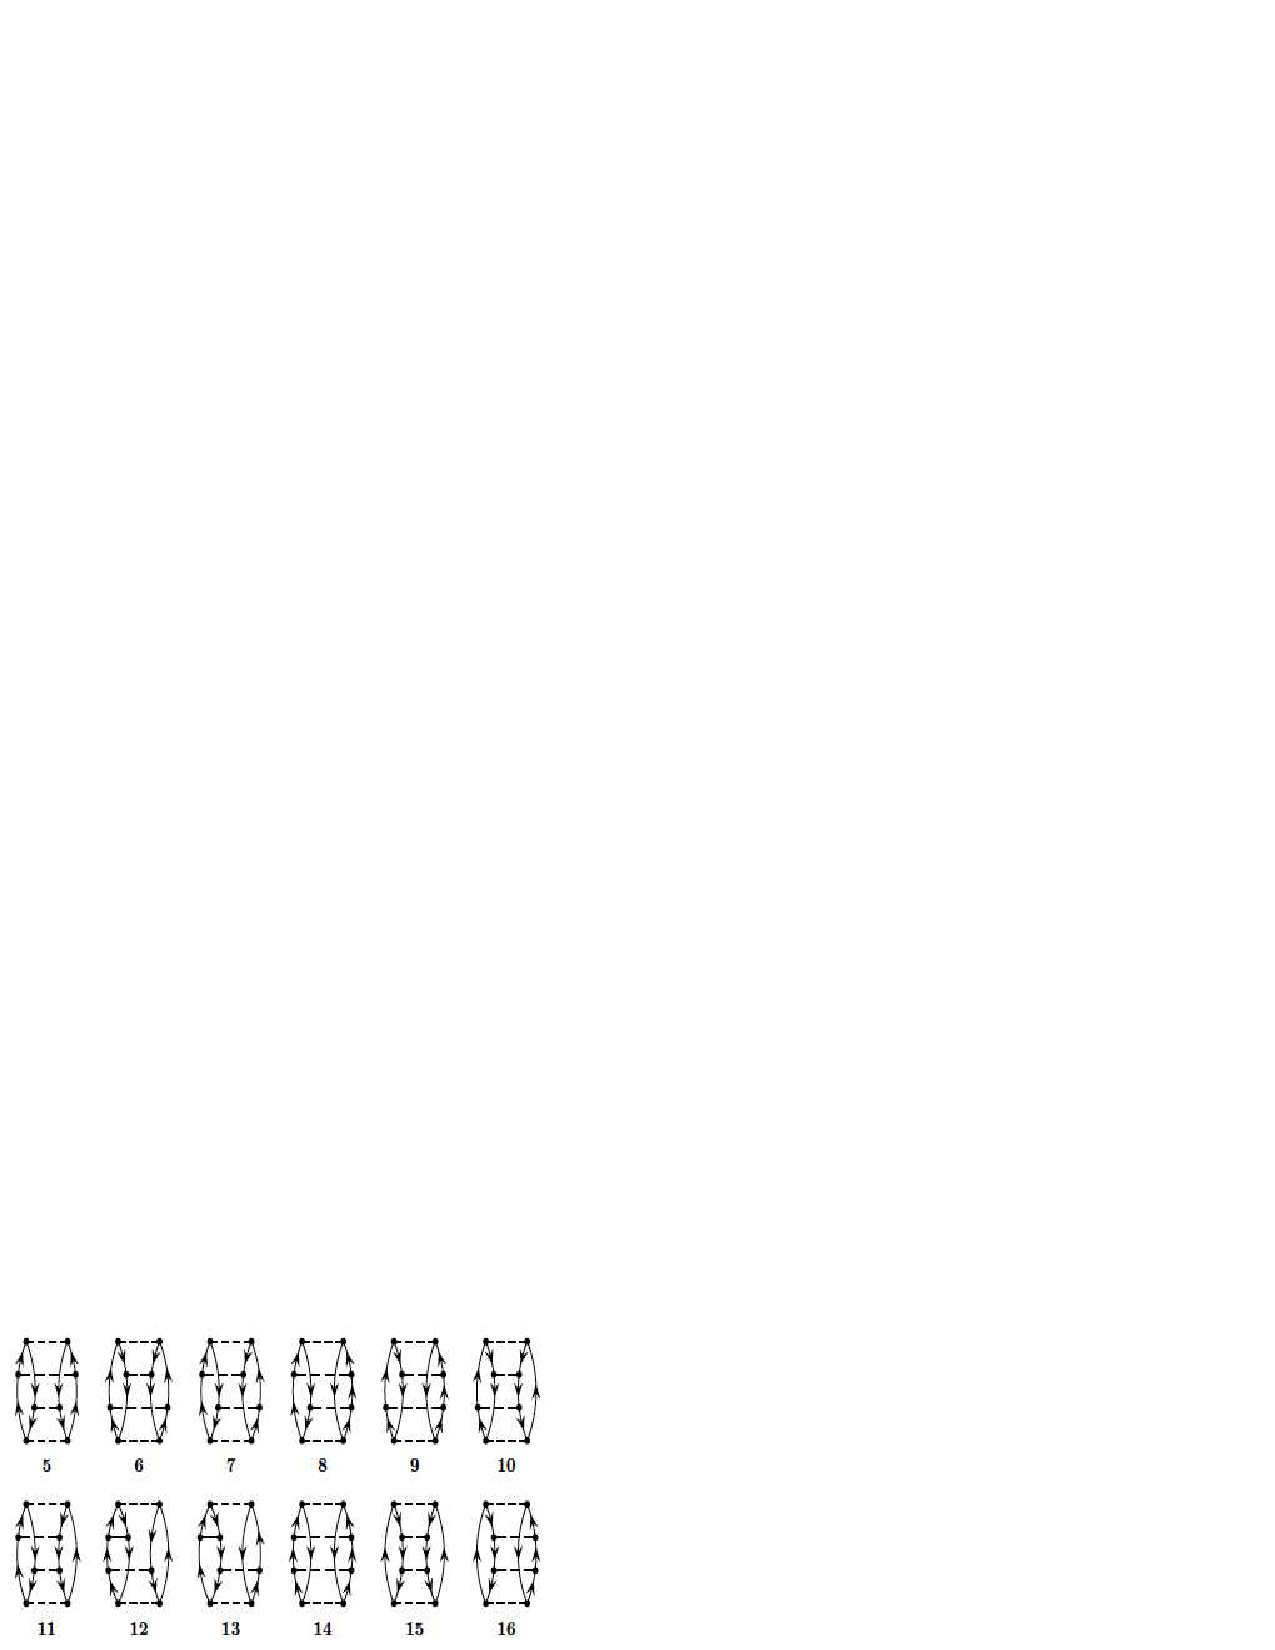
\includegraphics[width=0.6\linewidth]{fig-proj/2p2h.pdf}}
  \caption{
  Two-particle-two-hole excitations to fourth order. \label{fig:fourthorder2p2h}
  }
\end{figure}
%\clearpage % flush figures fig:fourthorder2p2h



\begin{figure}[t]
  \centerline{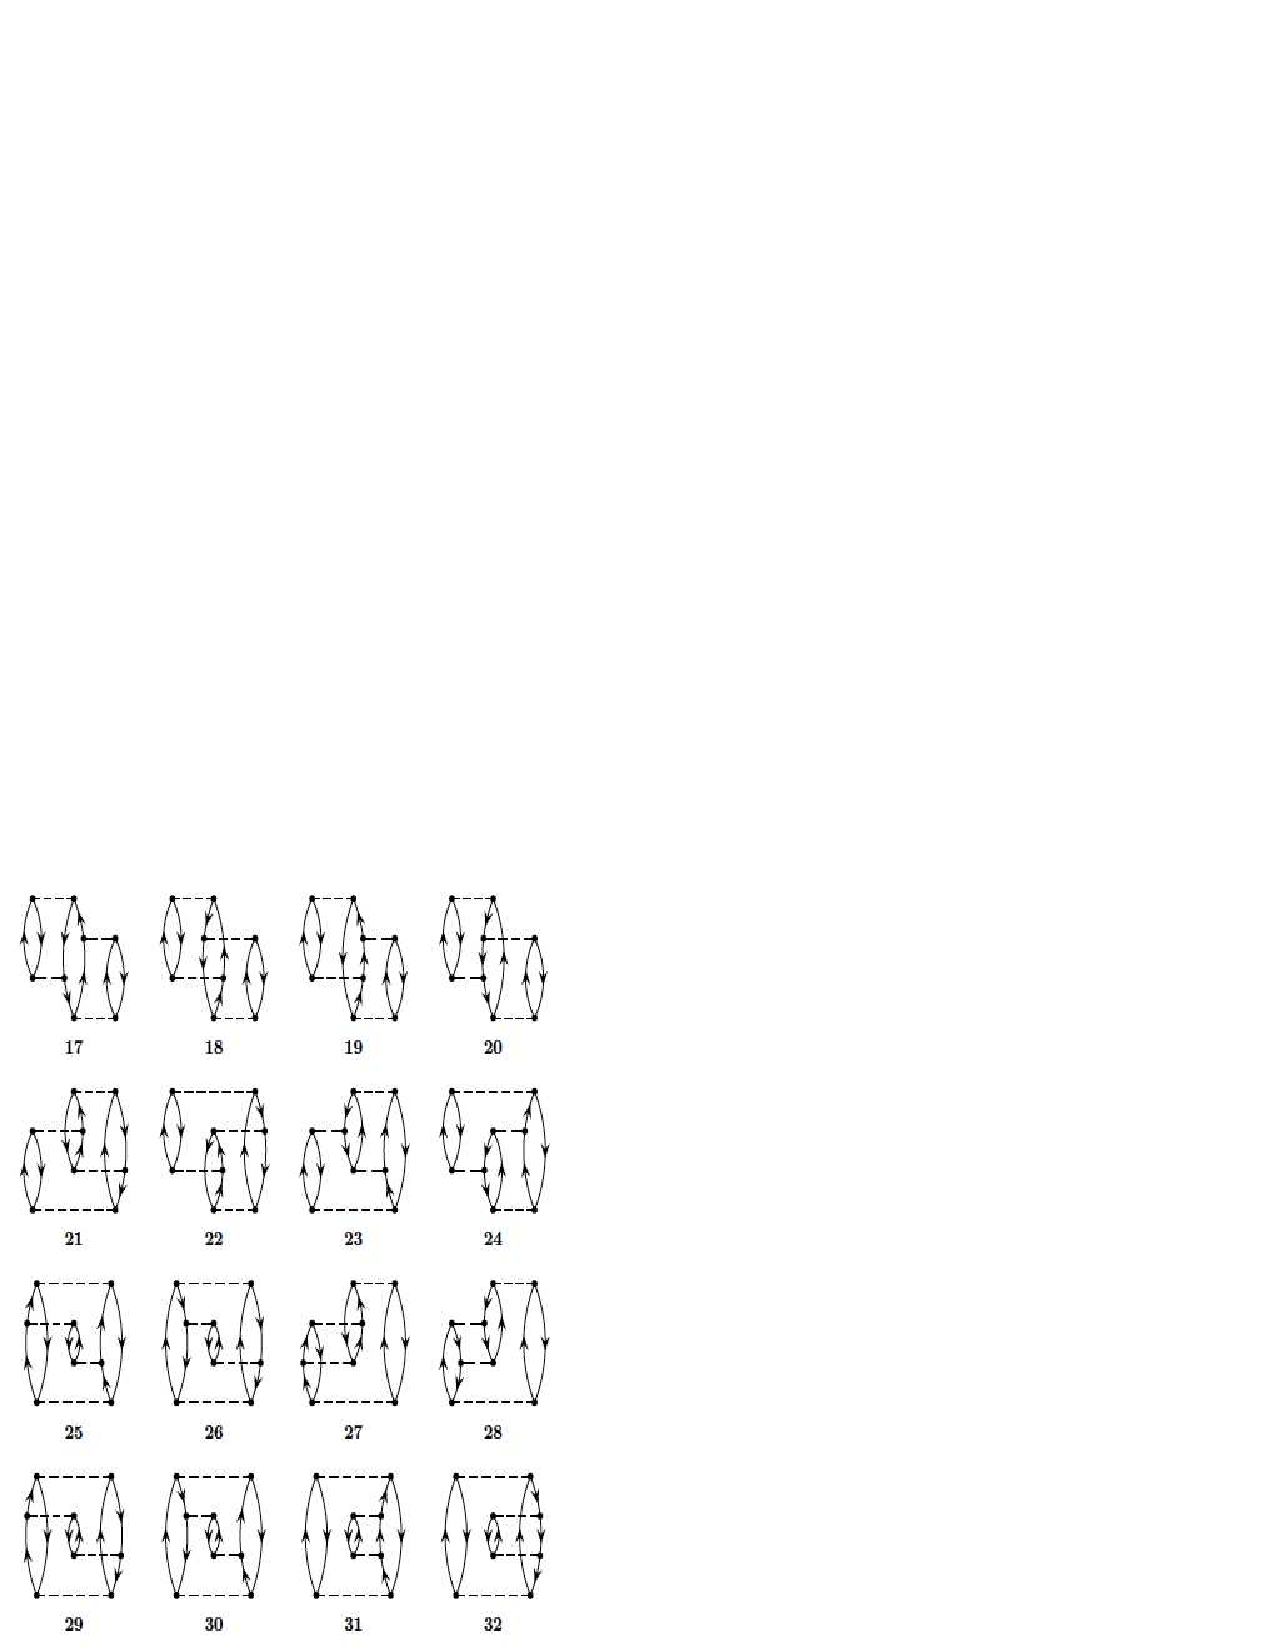
\includegraphics[width=0.6\linewidth]{fig-proj/3p3h.pdf}}
  \caption{
  Three-particle-three-hole excitations to fourth order. \label{fig:fourthorder3p3h}
  }
\end{figure}
%\clearpage % flush figures fig:fourthorder3p3h



\begin{figure}[t]
  \centerline{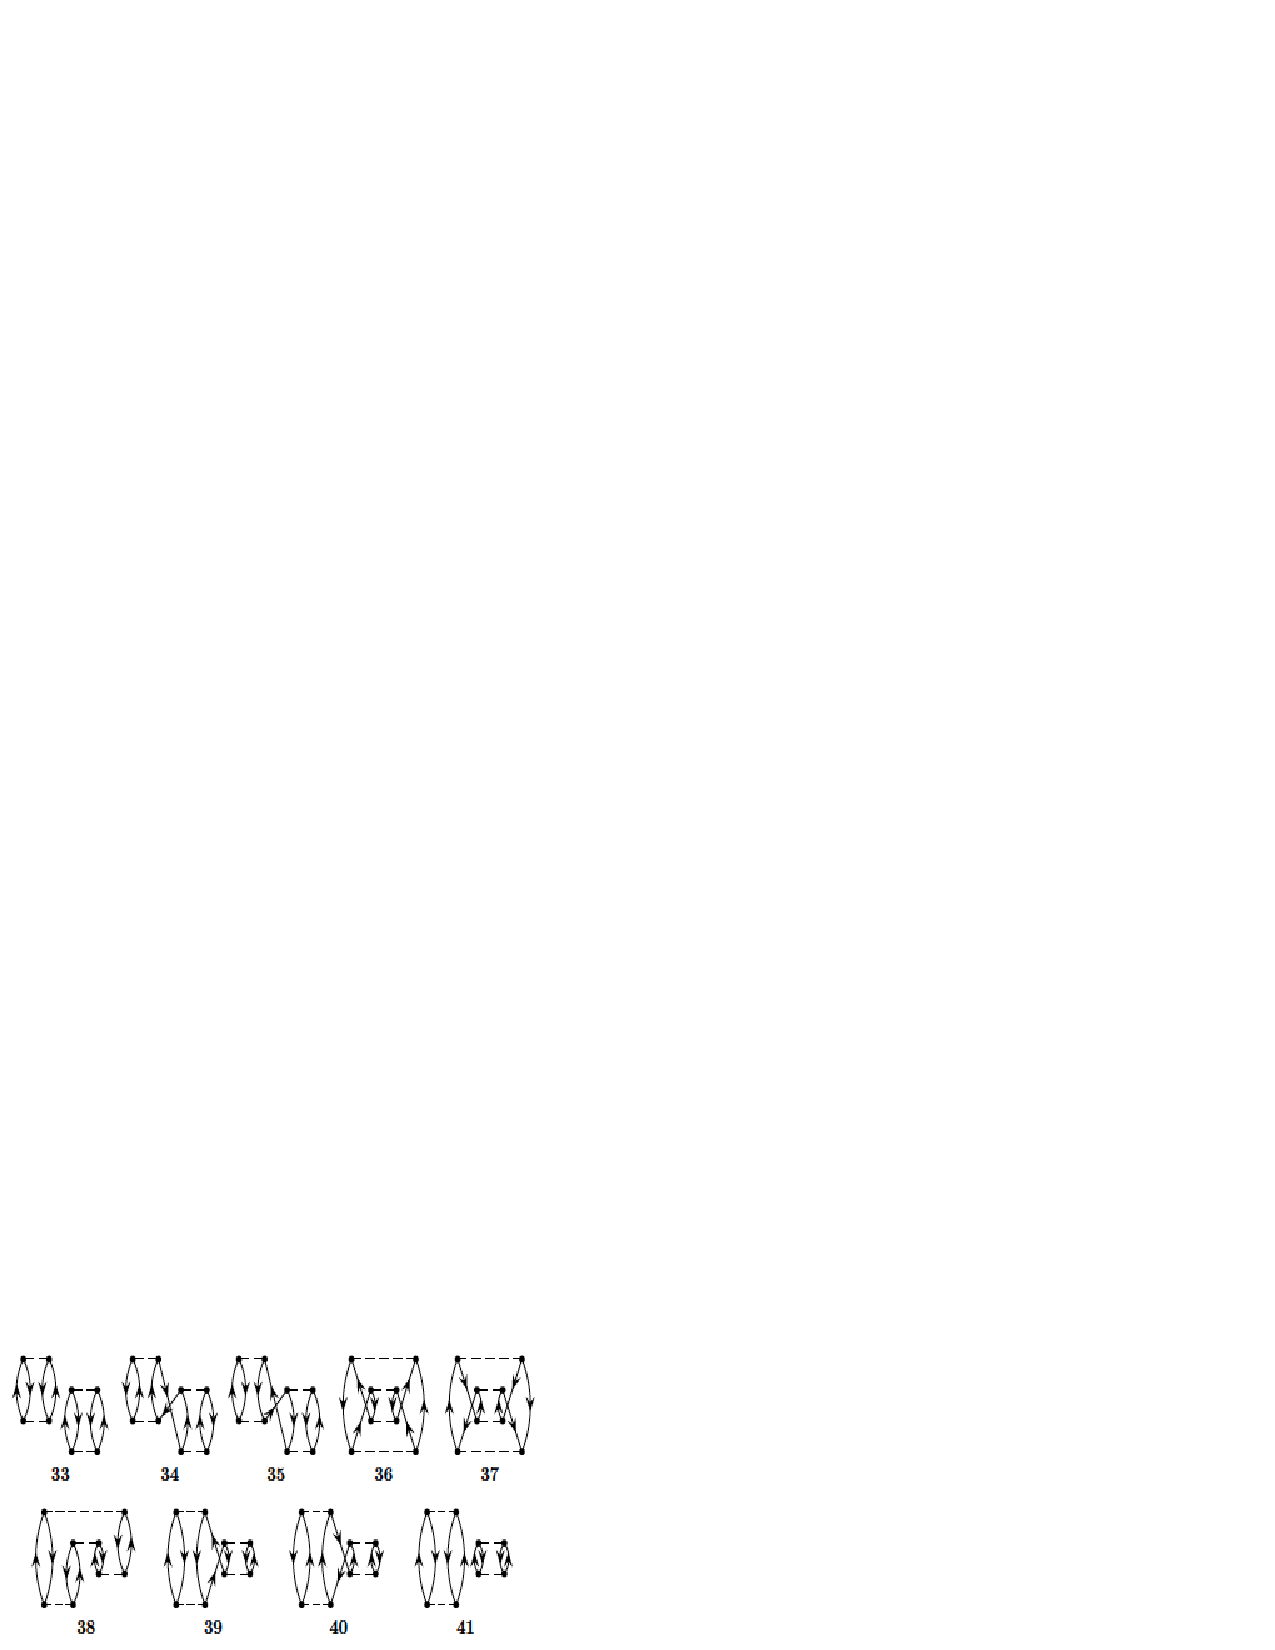
\includegraphics[width=0.6\linewidth]{fig-proj/4p4h.pdf}}
  \caption{
  Four-particle-four-hole excitations to fourth order. \label{fig:fourthorder4p4h}
  }
\end{figure}
%\clearpage % flush figures fig:fourthorder4p4h


Define first linked and unlinked diagrams and explain briefly Goldstone's linked diagram theorem.
Based on the linked diagram theorem and the form of the pairing Hamiltonian, which diagrams will contribute
to fourth order? 

Calculate the energy to fourth order with a canonical Hartree-Fock basis for $g\in [-1,1]$ and compare
with the full diagonalization case in exercise 2). Discuss the results.


% --- begin solution of exercise ---
\paragraph{Solution.}
The following Python program gives us the final results.
\bpypro
from sympy import *
from pylab import *

below_fermi = (0,1,2,3)
above_fermi = (4,5,6,7)

states = [(1,1),(1,-1),(2,1),(2,-1),(3,1),(3,-1),(4,1),(4,-1)]
N = 8
g = Symbol('g')



def h0(p,q):
	if p == q:
		p1, s1 = states[p]
		return (p1 - 1)	
	else:
		return 0

def f(p,q):
	if p == q:
		return 0

	s = h0(p,q)
	for i in below_fermi:
		s += assym(p,i,q,i)
	return s


def assym(p,q,r,s):
	p1, s1 = states[p]
	p2, s2 = states[q]
	p3, s3 = states[r]
	p4, s4 = states[s]

	if p1 != p2 or p3 != p4:
		return 0
	if s1 == s2 or s3 == s4:
		return 0
	if s1 == s3 and s2 == s4:
		return -g/2.
	if s1 == s4 and s2 == s3:
		return g/2.

def eps(holes, particles):
	E = 0
	for h in holes:
		p, s = states[h]
		E += (p-1)
	for p in particles:
		p, s = states[p]
		E -= (p-1)
	return E


# Diagram 3
# s = 0 
# for a in above_fermi:
# 	for b in above_fermi:
# 		for c in above_fermi:
# 			for i in below_fermi:
# 				for j in below_fermi:
# 					for k in below_fermi:
# 						s += assym(i,j,a,b)*assym(a,c,j,k)*assym(b,k,c,i)/eps((i,j),(a,b))/eps((k,j),(a,c))
# print s


# ga = linspace(-1,1,101)
# corr2 = []
# corr3 = []
# corrx = []


# Diagram 1
s1 = 0
for a in above_fermi:
	for b in above_fermi:
		for i in below_fermi:
			for j in below_fermi:
				s1 += 0.25*assym(a,b,i,j)*assym(i,j,a,b)/eps((i,j),(a,b))

# Diagram 4
s4 = 0
for a in above_fermi:
	for b in above_fermi:
		for c in above_fermi:
			for d in above_fermi:
				for i in below_fermi:
					for j in below_fermi:
						s4 += 0.125*assym(i,j,a,b)*assym(a,b,c,d)*assym(c,d,i,j)/eps((i,j),(a,b))/eps((i,j),(c,d))

# Diagram 5
s5 = 0
for a in above_fermi:
	for b in above_fermi:
		for i in below_fermi:
			for j in below_fermi:
				for k in below_fermi:
					for l in below_fermi:
						s5 += 0.125*assym(i,j,a,b)*assym(k,l,i,j)*assym(a,b,k,l)/eps((i,j),(a,b))/eps((k,l),(a,b))

# Diagram 8 (simplified)
s8 = 0 
for a in above_fermi:
	for b in above_fermi:
		for i in below_fermi:
			for j in below_fermi:
				for k in below_fermi:
					s8 -= 0.5*assym(i,j,a,b)*assym(a,b,i,k)*f(k,j)/eps((i,j),(a,b))/eps((i,k),(a,b))

# Diagram 9 (simplified)
s9 = 0 
for a in above_fermi:
	for b in above_fermi:
		for c in above_fermi:
			for i in below_fermi:
				for j in below_fermi:
					s9 += 0.5*assym(i,j,a,b)*assym(a,c,i,j)*f(b,c)/eps((i,j),(a,b))/eps((i,j),(a,c))


print s1
print s4
print s5
print s8
print s9

s_5 =  -0.0291521990740741*g**4
s14 =  -0.0308883101851853*g**4
s34 =  0.0163049768518519*g**4
s36 =  -0.0145760995370371*g**4
s38 =  -0.0201099537037037*g**4
s39 =  0.0176938657407407*g**4

ga = linspace(-1,1,10001)
e1 = []
corr2 = []
corr3 = []
corr4 = []
for g_val in ga:
	H1 = matrix([[2-g_val , -g_val/2.,  -g_val/2., -g_val/2., -g_val/2.,     0], 
		        [-g_val/2.,   4-g_val,  -g_val/2., -g_val/2.,    0., -g_val/2.],
		        [-g_val/2., -g_val/2.,    6-g_val,     0, -g_val/2., -g_val/2.],
				[-g_val/2., -g_val/2.,      0,   6-g_val, -g_val/2., -g_val/2.],
				[-g_val/2.,     0,  -g_val/2., -g_val/2.,   8-g_val, -g_val/2.],
				[0    , -g_val/2.,  -g_val/2., -g_val/2., -g_val/2.,  10-g_val]]) 

	u1, v1 = linalg.eig(H1)
	e1.append(min(u1))

	corr2.append((s1).subs(g,g_val))
	corr3.append((s1+s4+s5).subs(g,g_val))
	corr4.append((s1+s4+s5+2*s_5+2*s14+2*s34+2*s36+s38+2*s39).subs(g,g_val))

exact = e1 - (2-ga)

plot(ga, exact, linewidth=2.0)
plot(ga, corr2, linewidth=2.0)
plot(ga, corr3, linewidth=2.0)
plot(ga, corr4, linewidth=2.0)
xlabel(r'Interaction strength, $g$', fontsize=16)
ylabel(r'Correlation energy', fontsize=16)
axis([-1,1,-0.5,0.05])
grid()
legend(["Exact", "2. order MPBT", "3. order MPBT", "4. order MPBT"], 'lower left')
savefig("perturbationtheory.pdf")
show()
error1 = zeros(len(exact))
error2 = zeros(len(exact))
error3 = zeros(len(exact))

for i in range(len(exact)):
	error1[i] = abs(float(exact[i]-corr2[i]))
	error2[i] = abs(float(exact[i]-corr3[i]))
	error3[i] = abs(float(exact[i]-corr4[i]))

error1 = array(error1)
error2 = array(error2)
error3 = array(error3)
print type(error1)

plot(ga, log10(error1))
plot(ga, log10(error2))
plot(ga, log10(error3))
xlabel(r"Strength of interaction, $g$", fontsize=16)
ylabel(r"Error, $\log_{\rm 10}({\rm abs}({\rm error})$", fontsize=16)
legend(["2. order MPBT", "3. order MPBT", "4. order MPBT"], 'lower left')
grid()
savefig("logerror.pdf")
show()
\epypro

% --- end solution of exercise ---

\end{doconceexercise}
% --- end exercise ---




% --- begin exercise ---
\begin{doconceexercise}
\refstepcounter{doconceexercisecounter}

\subsection*{Project \thedoconceexercisecounter: Coupled cluster calculations with doubles excitations only for the pairing model}


This project serves as a continuation to the pairing model with the aim being to solve the same problem but now by developing
a program that implements the coupled cluster method with double excitations only. In doing so you will find it convenient to write 
classes which define the single-particle basis and the Hamiltonian. Your functions that solve the coupled cluster equations will then just need to set up variables which point to interaction elements and single-particle states with their pertinent quantum numbers. Use for example the setup discussed in the FCI lectures for the pairing model.


\subex{a)}
Explain why no single excitations are involved in this model.

\subex{b)}
Set up the coupled cluster equations for doubles excitations and convince yourself about their meaning and correctness.

\subex{c)}
Write a class which holds single-particle data like specific quantum numbers, single-particle Hamiltonian etc. Write also a class which sets up and stores two-body matrix elements defined by the single-particle states.  Write thereafter functions/classes which implement the coupled cluster method with doubles only.

\subex{d)}
Compare your results with those from the exact diagonalization with and without the $4p4h$ excitation. Compare also your results to perturbation theory at different orders, in particular to second order. Discuss your results.

\end{doconceexercise}
% --- end exercise ---




% --- begin exercise ---
\begin{doconceexercise}
\refstepcounter{doconceexercisecounter}

\subsection*{Project \thedoconceexercisecounter: Coupled cluster calculations with doubles excitations only for infinite nuclear matter}



\subex{a)}
Explain why we don't have single excitations in infinite matter.

\subex{b)}
Set up the relavent quantum numbers for a cartesian basis with plane waves in three dimensions. Make the according changes to the code you developed in connection with the pairing model. Implement periodic boundary conditions.

\subex{c)}
Replace the two-body interaction from the pairing model with the Minnesota potential model (to be inserted here later).

\subex{d)}
Use the program you developed in connection with the pairing model to perform coupled cluster calculations in infinite matter with doubles excitations.
Perform coupled cluster calculations for infinite nuclear matter with the Minnesota interaction for different particle numbers (to be inserted later).
Limit yourself to two-particle and two-hole intermediate excitations only.

\subex{e)}
Compare the two-particle only excitations with a finite number of particles with results obtained with Brueckner-Hartree-Fock calculations in the thermodynamic limit. Comment your results

\subex{f)}
The final challenge is to include particle-hole excitations and compare the results with those from Diffusion Monte Carlo calculations (insert ref here).
This part can be included in the final project.

\end{doconceexercise}
% --- end exercise ---




% --- begin exercise ---
\begin{doconceexercise}
\refstepcounter{doconceexercisecounter}

\subsection*{Project \thedoconceexercisecounter: Coupled cluster calculations with doubles excitations only for finite nuclei}



\subex{a)}
Add material here

\end{doconceexercise}
% --- end exercise ---




% --- begin exercise ---
\begin{doconceexercise}
\refstepcounter{doconceexercisecounter}

\subsection*{Project \thedoconceexercisecounter: Green's function calculations with doubles excitations only for the pairing model}



\subex{a)}
Explain why no single excitations are involved in this model.

\subex{b)}
Set up the Green's function equations for doubles excitations and convince yourself about their meaning and correctness.

\subex{c)}
Write a class which holds single-particle data like specific quantum numbers, single-particle Hamiltonian etc. Write also a class which sets up and stores two-body matrix elements defined by the single-particle states.  Write thereafter functions/classes which implement the Green's function method with doubles only.

\subex{d)}
Compare your results with those from the exact diagonalization with and without the $4p4h$ excitation. Compare also your results to perturbation theory at different orders, in particular to second order. Discuss your results. If other groups are solving the same problem with the coupled cluster method, discuss these results as well.

\end{doconceexercise}
% --- end exercise ---




% --- begin exercise ---
\begin{doconceexercise}
\refstepcounter{doconceexercisecounter}

\subsection*{Project \thedoconceexercisecounter: Green's function calculations with doubles excitations only for infinite nuclear matter}



\subex{a)}
Explain why we don't have single excitations in infinite matter.

\subex{b)}
Set up the relavent quantum numbers for a cartesian basis with plane waves in three dimensions. Make the according changes to the code you developed in connection with the pairing model. Implement periodic boundary conditions.

\subex{c)}
Replace the two-body interaction from the pairing model with the Minnesota potential model (to be inserted here later).

\subex{d)}
Use the program you developed in connection with the pairing model to perform Green's function calculations in infinite matter with doubles excitations.
Perform Green's function calculations for infinite nuclear matter with the Minnesota interaction for different particle numbers (to be inserted later).
Limit yourself to two-particle and two-hole intermediate excitations only.

\subex{e)}
Compare the two-particle only excitations with a finite number of particles with results obtained with Brueckner-Hartree-Fock calculations in the thermodynamic limit. Comment your results

\end{doconceexercise}
% --- end exercise ---




% --- begin exercise ---
\begin{doconceexercise}
\refstepcounter{doconceexercisecounter}

\subsection*{Project \thedoconceexercisecounter: Green's function calculations with doubles excitations only for finite nuclei}



\subex{a)}
Add material here

























\end{doconceexercise}
% --- end exercise ---


% ------------------- end of main content ---------------


% #ifdef PREAMBLE
\printindex

\end{document}
% #endif

